\documentclass[journal]{IEEEtran}
\usepackage{amsmath,amssymb}
\usepackage{graphicx}
\usepackage{booktabs}
\usepackage{url}
\usepackage{microtype}
\renewcommand{\thefigure}{S\arabic{figure}}
\renewcommand{\thetable}{S\arabic{table}}
\newcommand{\ours}{FORTRESS-FL}

\begin{document}
\title{Supplementary Material for\\ ``Certified Federated Unlearning for IoT: Ledger-Anchored Revocation with Anytime-Valid Forgetting Certificates''}
\author{Quang-Vinh Dang}
\maketitle

\section{Setup and cost model}
All experiments are produced by the scripts in the repository (\texttt{experiments/unlearning\_experiments.py}, \texttt{unlearning\_real.py}, \texttt{unlearning\_new.py}); tables below are written from the result files by \texttt{paper/make\_supp\_tables.py}.

\textbf{Training.} Binary logistic loss, full-batch local gradient, update clipping at norm 1, learning rate 1, $T=60$ rounds, participation $p=0.6$ (independent per client and round), reputation rate 0.1 and penalty 0.2, Pedersen commitments with 512-bit group, spectral split gated by a separation margin of 0.25, no differential-privacy noise unless stated. Synthetic fleet: 60 clients, $d=1024$, 12 real records and 6 canary pairs per client, Dirichlet($\alpha{=}1$) over ten latent classes, 8\% label noise. UCI HAR: 30 subjects, 40 records each. N-BaIoT: nine devices, five sites each, 40 records each, features $\operatorname{sign}(x)\log(1+|x|)$ standardised. The MLP has 32 tanh hidden units. Test records are held out per client. Audits use $\epsilon=0.2$, $\alpha=0.05$ and a reveal order drawn from a fixed seed.

\textbf{Cost model.} A client round with $n$ records costs $n\cdot f$ FLOPs ($f=4d$ for the linear model, $6P$ for an MLP with $P$ parameters), uploads $4P+64$ bytes (float32 update and a 512-bit commitment) and downloads $4P$ bytes. Energy is $e_{\rm flop}\cdot\text{FLOPs}+e_{\rm bit}\cdot 8\cdot\text{bytes}$ with $e_{\rm flop}=1$~nJ and $e_{\rm bit}=100$~nJ; these are assumed constants, not measurements. With them radio traffic dominates, so energy follows bytes. Canary reveal sends $2m(d{+}1)\cdot 4$ bytes per revoked client once.

\section{Additional figures}
\begin{figure}[h]
\centering
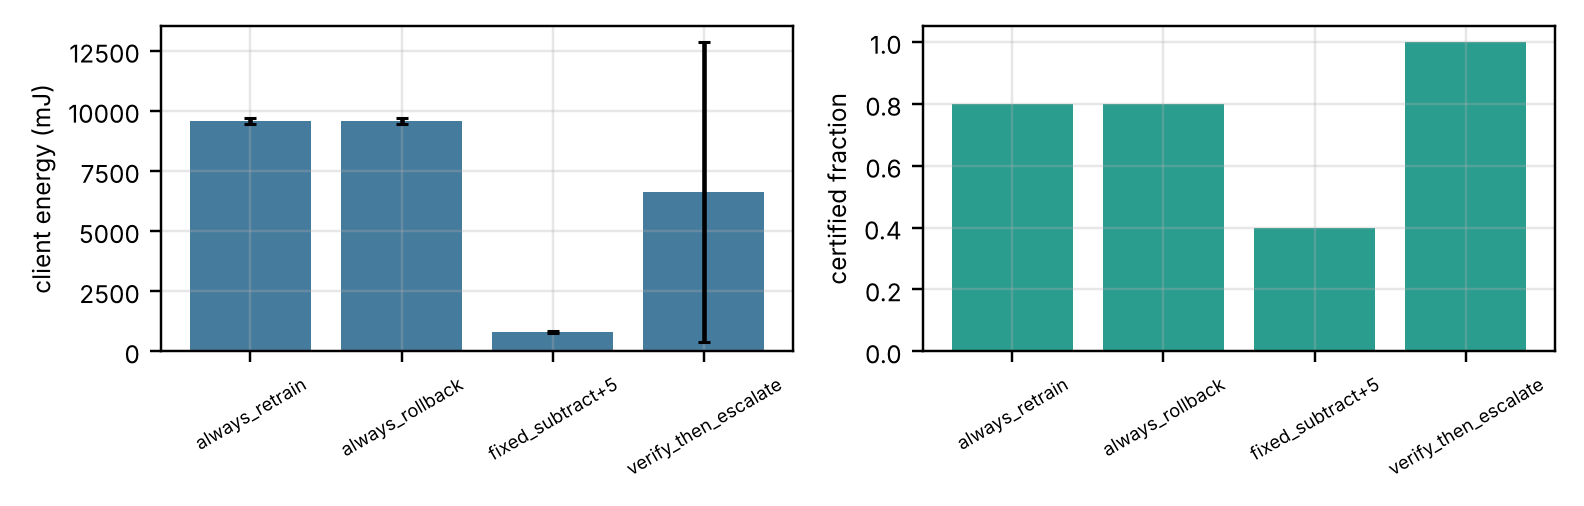
\includegraphics[width=\columnwidth]{cert_escalation.png}
\caption{Synthetic fleet, wave of 20 clients (10 seeds): mean client energy (bars, s.d. as error bars) and share of waves certified for the verify-then-escalate ladder, always retraining, always rollback and a fixed subtract+5 policy.}\label{fig:s_esc}
\end{figure}
\begin{figure}[h]
\centering
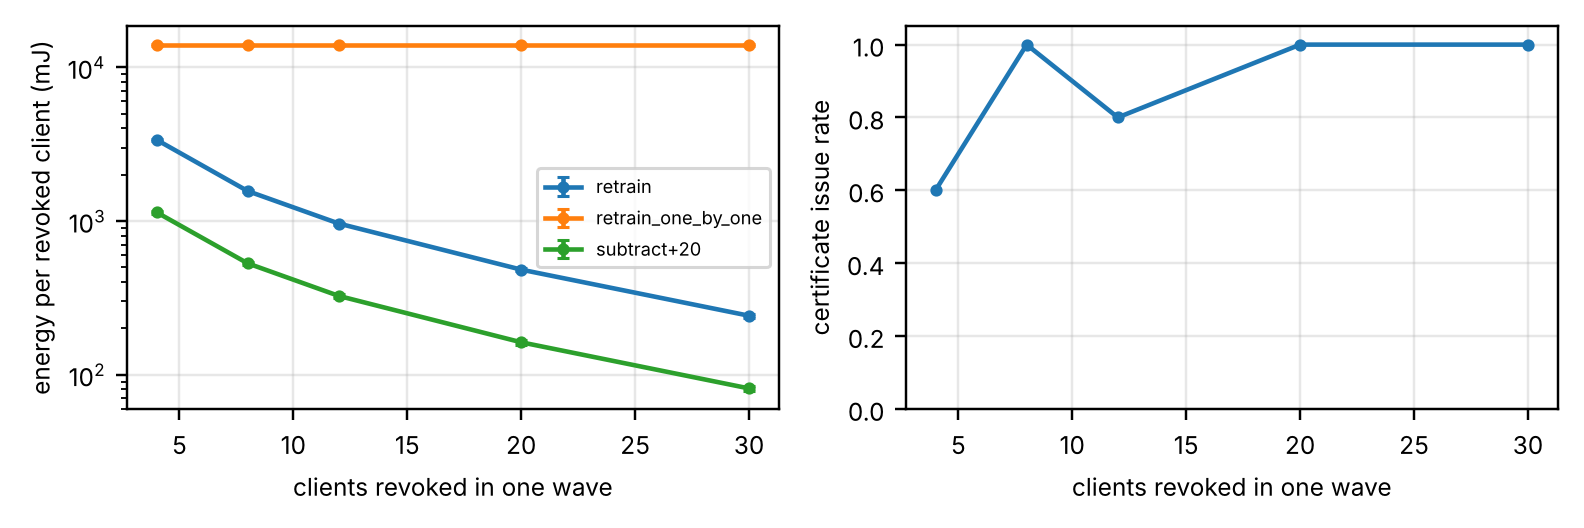
\includegraphics[width=\columnwidth]{cert_wave.png}
\caption{Synthetic fleet: energy per revoked client versus wave size (left; ``one by one'' is measured on three requests and extrapolated) and issue rate of the certificate for the retrained model (right, 5 seeds).}\label{fig:s_wave}
\end{figure}
\begin{figure}[h]
\centering
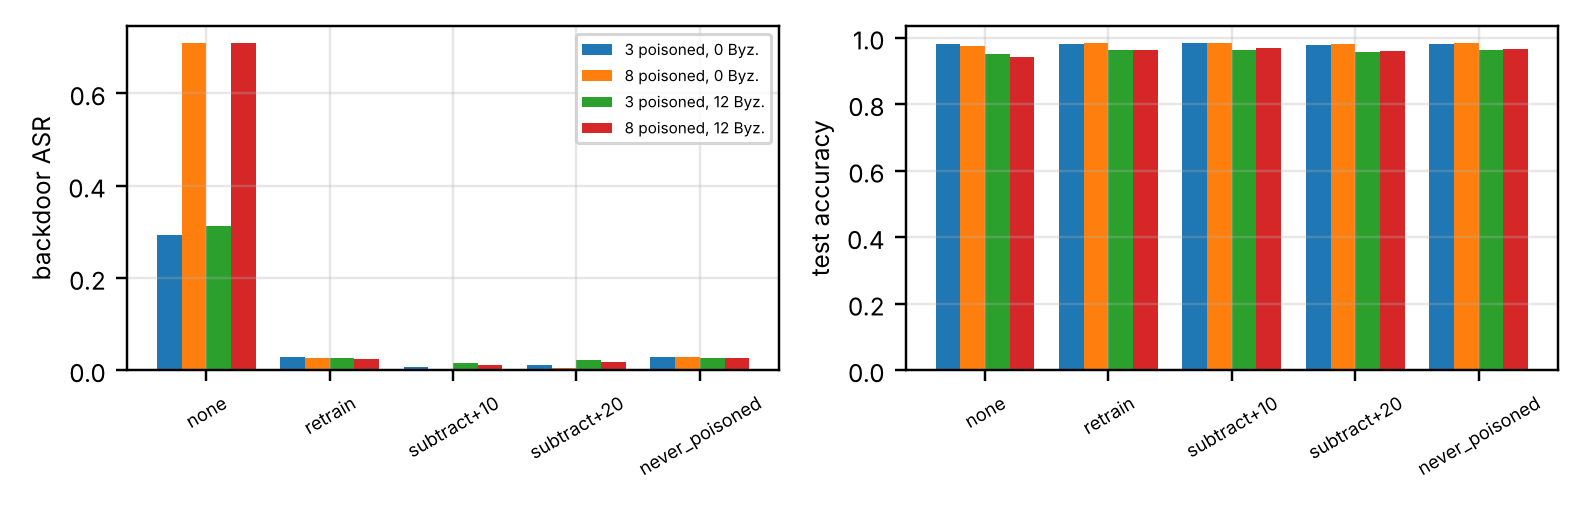
\includegraphics[width=\columnwidth]{cert_poison.png}
\caption{Synthetic fleet, backdoor success rate and test accuracy before and after unlearning, with 3 or 8 poisoned clients in the wave and with 0 or 12 Byzantine sign-flipping clients (5 seeds).}\label{fig:s_poison}
\end{figure}
\begin{figure}[h]
\centering
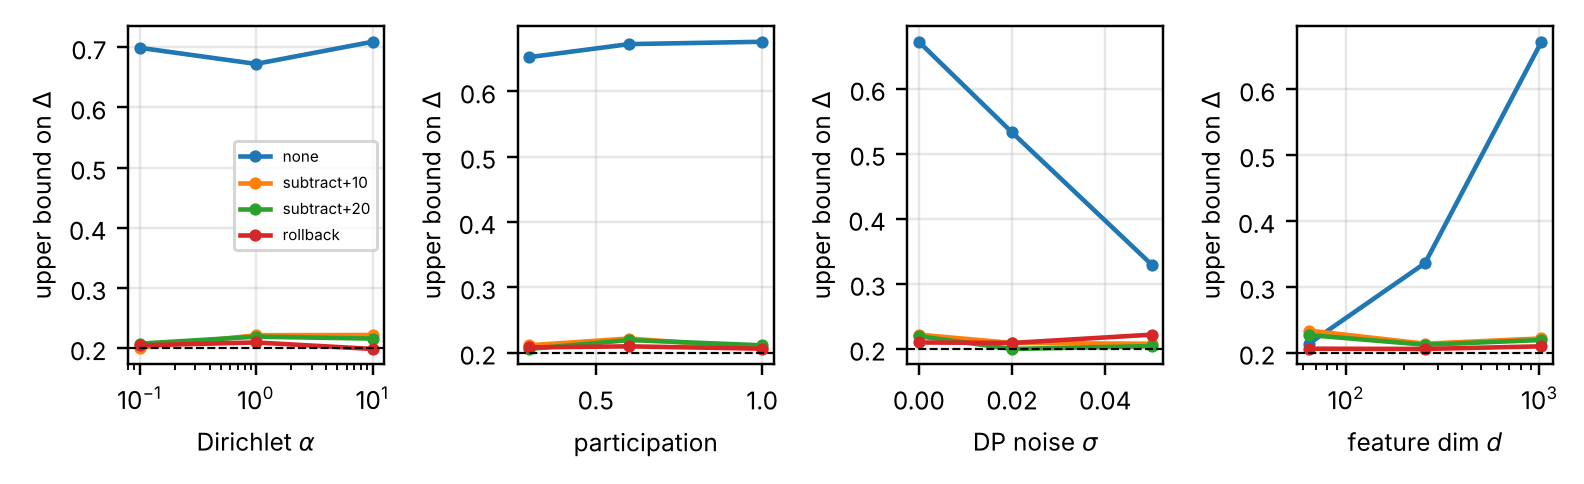
\includegraphics[width=\columnwidth]{cert_sweeps.png}
\caption{Synthetic fleet: upper bound on the residual advantage against the Dirichlet parameter, participation rate, DP noise and feature dimension for the un-unlearned model and three operators (5 seeds). Dashed: $\epsilon=0.2$.}\label{fig:s_sweeps}
\end{figure}
\begin{figure*}[h]
\centering
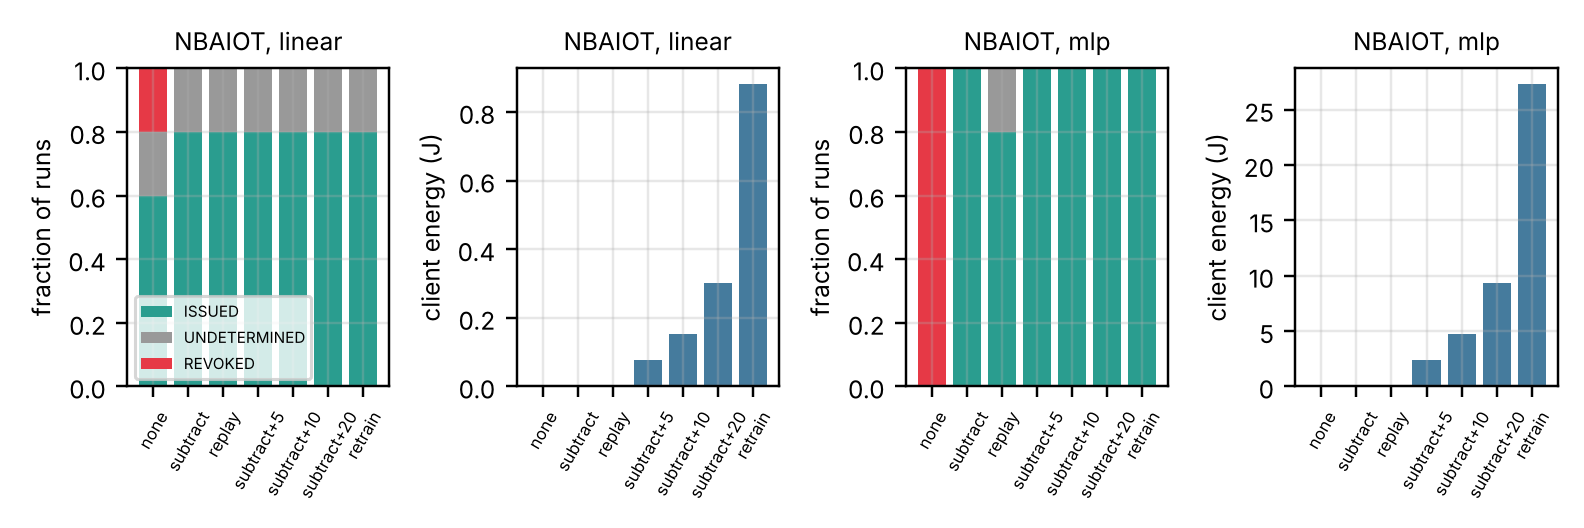
\includegraphics[width=0.92\textwidth]{nbaiot_methods.png}
\caption{N-BaIoT (45 clients, wave of 15, 5 seeds): certificate outcomes and client energy per operator for the linear model and the MLP.}\label{fig:s_nb}
\end{figure*}
\begin{figure}[h]
\centering
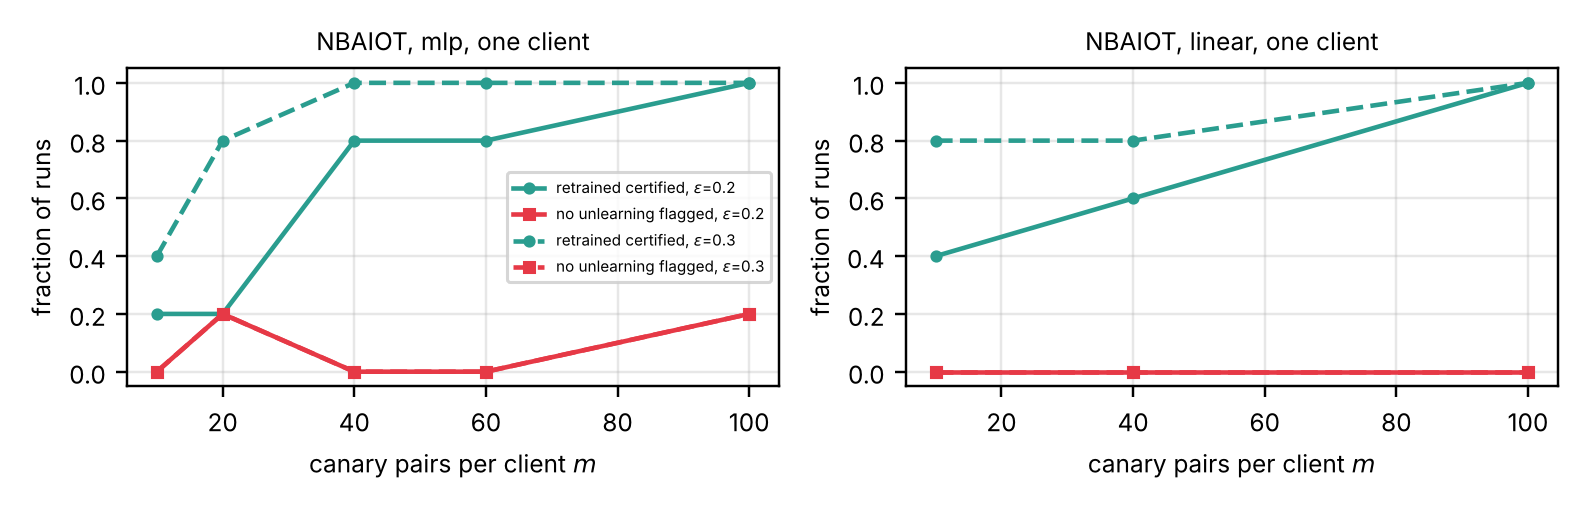
\includegraphics[width=\columnwidth]{nbaiot_per_client.png}
\caption{N-BaIoT, one revoked client: share of runs in which the retrained model is certified and the un-unlearned model is flagged, against canary pairs per client. The audit has little power at these model sizes.}\label{fig:s_nbpc}
\end{figure}

\section{Additional tables}
\begin{table}[h]
\centering
\caption{Synthetic fleet, one wave of 20 of 60 clients, 10 seeds. I/U/R: certificate issued, undetermined, revoked. $\Delta_{\rm up}$: mean upper bound on the residual advantage.}\label{tab:s_methods}
\footnotesize
\setlength{\tabcolsep}{3pt}
\begin{tabular}{@{}lcccccc@{}}
\toprule
Operator & I/U/R & Acc. & $\Delta_{\rm up}$ & Rounds & MB & Energy (J) \\
\midrule
none & 0/0/10 & 0.981 & 0.667 & 0 & 0.00 & 0.00 \\
subtract & 4/1/5 & 0.620 & 0.243 & 0 & 0.00 & 0.00 \\
replay & 4/1/5 & 0.621 & 0.252 & 0 & 0.00 & 0.00 \\
subtract+5 & 4/1/5 & 0.983 & 0.249 & 5 & 1.00 & 0.81 \\
subtract+10 & 4/3/3 & 0.982 & 0.226 & 10 & 2.03 & 1.64 \\
subtract+20 & 6/3/1 & 0.981 & 0.212 & 20 & 4.00 & 3.24 \\
rollback & 8/2/0 & 0.983 & 0.212 & 60 & 11.84 & 9.58 \\
retrain & 8/2/0 & 0.983 & 0.212 & 60 & 11.84 & 9.58 \\
\bottomrule
\end{tabular}
\end{table}

\begin{table}[h]
\centering
\caption{Calibration: the un-unlearned model (should be flagged) and the exactly retrained model (should not).}\label{tab:s_calib}
\footnotesize
\setlength{\tabcolsep}{3pt}
\begin{tabular}{@{}lllcc@{}}
\toprule
Data & Model & Model state & Runs & I/U/R \\
\midrule
synthetic & linear & none & 40 & 0/0/40 \\
synthetic & linear & retrain & 40 & 40/0/0 \\
HAR & linear & none & 60 & 0/0/60 \\
HAR & linear & retrain & 60 & 49/11/0 \\
HAR & mlp & none & 60 & 0/0/60 \\
HAR & mlp & retrain & 60 & 51/7/2 \\
N-BaIoT & linear & none & 60 & 42/9/9 \\
N-BaIoT & linear & retrain & 60 & 55/3/2 \\
N-BaIoT & mlp & none & 60 & 14/11/35 \\
N-BaIoT & mlp & retrain & 60 & 54/6/0 \\
\bottomrule
\end{tabular}
\end{table}

\begin{table}[h]
\centering
\caption{Real data, a wave of one third of the clients, 5 seeds.}\label{tab:s_real}
\footnotesize
\setlength{\tabcolsep}{3pt}
\begin{tabular}{@{}lllcccc@{}}
\toprule
Data & Model & Operator & I/U/R & Acc. & Rounds & Energy (J) \\
\midrule
HAR & linear & none & 0/0/5 & 0.999 & 0 & 0.00 \\
HAR & linear & subtract & 2/2/1 & 0.991 & 0 & 0.00 \\
HAR & linear & replay & 2/1/2 & 0.991 & 0 & 0.00 \\
HAR & linear & subtract+5 & 2/2/1 & 0.998 & 5 & 0.22 \\
HAR & linear & subtract+10 & 2/2/1 & 0.998 & 10 & 0.46 \\
HAR & linear & subtract+20 & 3/1/1 & 0.998 & 20 & 0.91 \\
HAR & linear & retrain & 3/2/0 & 0.998 & 60 & 2.69 \\
HAR & mlp & none & 0/0/5 & 0.999 & 0 & 0.00 \\
HAR & mlp & subtract & 3/2/0 & 0.995 & 0 & 0.00 \\
HAR & mlp & replay & 3/2/0 & 0.995 & 0 & 0.00 \\
HAR & mlp & subtract+5 & 4/1/0 & 0.998 & 5 & 7.21 \\
HAR & mlp & subtract+10 & 4/1/0 & 0.998 & 10 & 14.90 \\
HAR & mlp & subtract+20 & 4/1/0 & 0.998 & 20 & 29.24 \\
HAR & mlp & retrain & 4/1/0 & 0.999 & 60 & 86.48 \\
N-BaIoT & linear & none & 3/1/1 & 0.996 & 0 & 0.00 \\
N-BaIoT & linear & subtract & 4/1/0 & 0.871 & 0 & 0.00 \\
N-BaIoT & linear & replay & 4/1/0 & 0.942 & 0 & 0.00 \\
N-BaIoT & linear & subtract+5 & 4/1/0 & 0.960 & 5 & 0.08 \\
N-BaIoT & linear & subtract+10 & 4/1/0 & 0.995 & 10 & 0.15 \\
N-BaIoT & linear & subtract+20 & 4/1/0 & 0.996 & 20 & 0.30 \\
N-BaIoT & linear & retrain & 4/1/0 & 0.995 & 60 & 0.88 \\
N-BaIoT & mlp & none & 0/0/5 & 0.997 & 0 & 0.00 \\
N-BaIoT & mlp & subtract & 5/0/0 & 0.962 & 0 & 0.00 \\
N-BaIoT & mlp & replay & 4/1/0 & 0.939 & 0 & 0.00 \\
N-BaIoT & mlp & subtract+5 & 5/0/0 & 0.996 & 5 & 2.38 \\
N-BaIoT & mlp & subtract+10 & 5/0/0 & 0.997 & 10 & 4.73 \\
N-BaIoT & mlp & subtract+20 & 5/0/0 & 0.997 & 20 & 9.35 \\
N-BaIoT & mlp & retrain & 5/0/0 & 0.997 & 60 & 27.36 \\
\bottomrule
\end{tabular}
\end{table}

\begin{table}[h]
\centering
\caption{Recovery policies (5 seeds). ``U'' counts undetermined and unpowered. Last column: worst run.}\label{tab:s_icr}
\footnotesize
\setlength{\tabcolsep}{3pt}
\begin{tabular}{@{}lllcccrr@{}}
\toprule
Data & Model & Policy & I/U/R & Acc. & Rounds & Mean J & Max J \\
\midrule
Synthetic & linear & retrain & 5/0/0 & 0.986 & 60.0 & 9.64 & 9.88 \\
Synthetic & linear & ladder & 5/0/0 & 0.985 & 41.0 & 6.68 & 13.81 \\
Synthetic & linear & icr\_q1.0 & 5/0/0 & 0.982 & 17.0 & 2.74 & 4.83 \\
Synthetic & linear & icr\_q0.5 & 4/1/0 & 0.982 & 16.0 & 1.30 & 4.81 \\
Synthetic & linear & icr\_q0.25 & 4/1/0 & 0.988 & 26.0 & 1.03 & 2.37 \\
HAR & linear & retrain & 3/2/0 & 0.999 & 60.0 & 2.69 & 2.74 \\
HAR & linear & ladder & 3/2/0 & 0.996 & 39.0 & 1.74 & 3.82 \\
HAR & linear & icr\_q1.0 & 4/1/0 & 0.996 & 24.0 & 1.07 & 2.63 \\
HAR & linear & icr\_q0.5 & 4/1/0 & 0.996 & 18.0 & 0.40 & 1.29 \\
HAR & linear & icr\_q0.25 & 3/2/0 & 0.996 & 27.0 & 0.34 & 0.75 \\
HAR & mlp & retrain & 4/1/0 & 0.999 & 60.0 & 86.48 & 88.12 \\
HAR & mlp & ladder & 4/1/0 & 0.997 & 18.0 & 25.56 & 119.58 \\
HAR & mlp & icr\_q1.0 & 4/1/0 & 0.997 & 13.0 & 18.54 & 84.50 \\
HAR & mlp & icr\_q0.5 & 4/1/0 & 0.997 & 13.0 & 9.02 & 41.47 \\
HAR & mlp & icr\_q0.25 & 4/1/0 & 0.997 & 13.0 & 5.09 & 23.63 \\
N-BaIoT & linear & retrain & 4/1/0 & 0.995 & 60.0 & 0.88 & 0.89 \\
N-BaIoT & linear & ladder & 1/4/0 & 0.980 & 24.0 & 0.36 & 1.25 \\
N-BaIoT & linear & icr\_q1.0 & 1/4/0 & 0.980 & 16.0 & 0.24 & 0.90 \\
N-BaIoT & linear & icr\_q0.5 & 1/4/0 & 0.981 & 15.0 & 0.11 & 0.45 \\
N-BaIoT & linear & icr\_q0.25 & 1/4/0 & 0.980 & 10.0 & 0.04 & 0.14 \\
N-BaIoT & mlp & retrain & 5/0/0 & 0.997 & 60.0 & 27.36 & 27.74 \\
N-BaIoT & mlp & ladder & 5/0/0 & 0.982 & 2.0 & 0.88 & 2.38 \\
N-BaIoT & mlp & icr\_q1.0 & 5/0/0 & 0.982 & 2.0 & 0.88 & 2.38 \\
N-BaIoT & mlp & icr\_q0.5 & 5/0/0 & 0.982 & 2.0 & 0.42 & 1.14 \\
N-BaIoT & mlp & icr\_q0.25 & 5/0/0 & 0.982 & 2.0 & 0.23 & 0.61 \\
\bottomrule
\end{tabular}
\end{table}

\begin{table}[h]
\centering
\caption{Canary design grid: share of runs (5 seeds) in which the audit flags the un-unlearned model.}\label{tab:s_power}
\footnotesize
\setlength{\tabcolsep}{3pt}
\begin{tabular}{@{}lllcccc@{}}
\toprule
Data & Model & $m$ & Scale & Flagged & $\Delta_{\rm up}$ & Acc. \\
\midrule
N-BaIoT & linear & 6 & 1 & 0.2 & 0.25 & 0.996 \\
N-BaIoT & linear & 12 & 1 & 0.6 & 0.22 & 0.996 \\
N-BaIoT & linear & 6 & 2 & 0.2 & 0.26 & 0.996 \\
N-BaIoT & linear & 12 & 2 & 0.6 & 0.21 & 0.967 \\
N-BaIoT & linear & 6 & 4 & 0.4 & 0.24 & 0.995 \\
N-BaIoT & linear & 12 & 4 & 0.6 & 0.21 & 0.932 \\
N-BaIoT & linear & 6 & 8 & 0.2 & 0.23 & 0.995 \\
N-BaIoT & linear & 12 & 8 & 0.8 & 0.22 & 0.967 \\
N-BaIoT & mlp & 6 & 1 & 1.0 & 0.36 & 0.997 \\
N-BaIoT & mlp & 12 & 1 & 1.0 & 0.35 & 0.997 \\
N-BaIoT & mlp & 6 & 2 & 1.0 & 0.50 & 0.997 \\
N-BaIoT & mlp & 12 & 2 & 1.0 & 0.52 & 0.997 \\
N-BaIoT & mlp & 6 & 4 & 1.0 & 0.57 & 0.997 \\
N-BaIoT & mlp & 12 & 4 & 1.0 & 0.59 & 0.997 \\
N-BaIoT & mlp & 6 & 8 & 1.0 & 0.46 & 0.997 \\
N-BaIoT & mlp & 12 & 8 & 1.0 & 0.56 & 0.997 \\
HAR & linear & 6 & 1 & 1.0 & 0.83 & 0.999 \\
HAR & linear & 12 & 1 & 1.0 & 0.65 & 0.999 \\
HAR & linear & 6 & 2 & 1.0 & 0.81 & 0.999 \\
HAR & linear & 12 & 2 & 1.0 & 0.61 & 0.999 \\
HAR & linear & 6 & 4 & 1.0 & 0.72 & 0.999 \\
HAR & linear & 12 & 4 & 1.0 & 0.61 & 0.999 \\
HAR & linear & 6 & 8 & 1.0 & 0.60 & 0.999 \\
HAR & linear & 12 & 8 & 1.0 & 0.56 & 0.999 \\
\bottomrule
\end{tabular}
\end{table}

\begin{table}[h]
\centering
\caption{Wave scheduler simulation, one year, 20 runs, deadline 30 days, power target 120 pairs.}\label{tab:s_sched}
\footnotesize
\setlength{\tabcolsep}{3pt}
\begin{tabular}{@{}llccccrc@{}}
\toprule
Req./day & Policy & Requests & Waves & Mean lat. & Max lat. & J/request & Underpowered \\
\midrule
0.2 & immediate & 73 & 66.2 & 0.5 & 1.0 & 2.48 & 1.00 \\
0.2 & batched & 73 & 11.1 & 17.2 & 29.9 & 0.42 & 1.00 \\
1 & immediate & 360 & 230.8 & 0.5 & 1.0 & 1.76 & 1.00 \\
1 & batched & 360 & 18.1 & 10.3 & 29.6 & 0.14 & 0.07 \\
4 & immediate & 1458 & 358.7 & 0.5 & 1.0 & 0.67 & 1.00 \\
4 & batched & 1458 & 66.8 & 2.8 & 27.5 & 0.13 & 0.01 \\
\bottomrule
\end{tabular}
\end{table}

\begin{table}[h]
\centering
\caption{Baselines on the MLP (5 seeds): marker success rate, loss-threshold membership AUC and our certificate outcome.}\label{tab:s_base}
\footnotesize
\setlength{\tabcolsep}{3pt}
\begin{tabular}{@{}llccc@{}}
\toprule
Data & Model state & Marker ASR & MIA AUC & Canary I/U/R \\
\midrule
HAR & none & 0.034 & 0.438 & 0/0/5 \\
HAR & retrain & 0.034 & 0.438 & 4/1/0 \\
HAR & subtract+20 & 0.030 & 0.438 & 4/1/0 \\
N-BaIoT & none & 0.395 & 0.426 & 0/0/5 \\
N-BaIoT & retrain & 0.432 & 0.416 & 5/0/0 \\
N-BaIoT & subtract+20 & 0.442 & 0.414 & 5/0/0 \\
\bottomrule
\end{tabular}
\end{table}

\begin{table}[h]
\centering
\caption{Provenance ledger on the synthetic fleet (3 seeds, 200 tamper trials each).}\label{tab:s_ledger}
\footnotesize
\setlength{\tabcolsep}{3pt}
\begin{tabular}{@{}lr@{}}
\toprule
Quantity & Value \\
\midrule
records (60 rounds) & 61 \\
ledger size (kB) & 101 \\
bytes per round & 1652 \\
ledger / update traffic & 0.011 \\
chain verification (ms) & 1.6 \\
Merkle proof check ($\mu$s) & 4.8 \\
proof length (hashes) & 5.7 \\
tampering detected & 1.00 \\
checkpoints (kB) & 417 \\
stored updates (kB) & 15154 \\
\bottomrule
\end{tabular}
\end{table}


\section{Reproduction}
\begin{verbatim}
pip install -r requirements.txt
python experiments/unlearning_experiments.py   # synthetic
python experiments/unlearning_real.py --dataset har
python experiments/prepare_nbaiot.py           # once
python experiments/unlearning_real.py --dataset nbaiot
python experiments/unlearning_new.py           # ICR, twins, ...
python experiments/fig_new.py
python paper/make_supp_tables.py
python tests/test_unlearning.py
\end{verbatim}
\end{document}
